% Replace the reserved Figure 1 placeholder in main.tex after review.
\begin{figure*}[t]
  \centering
  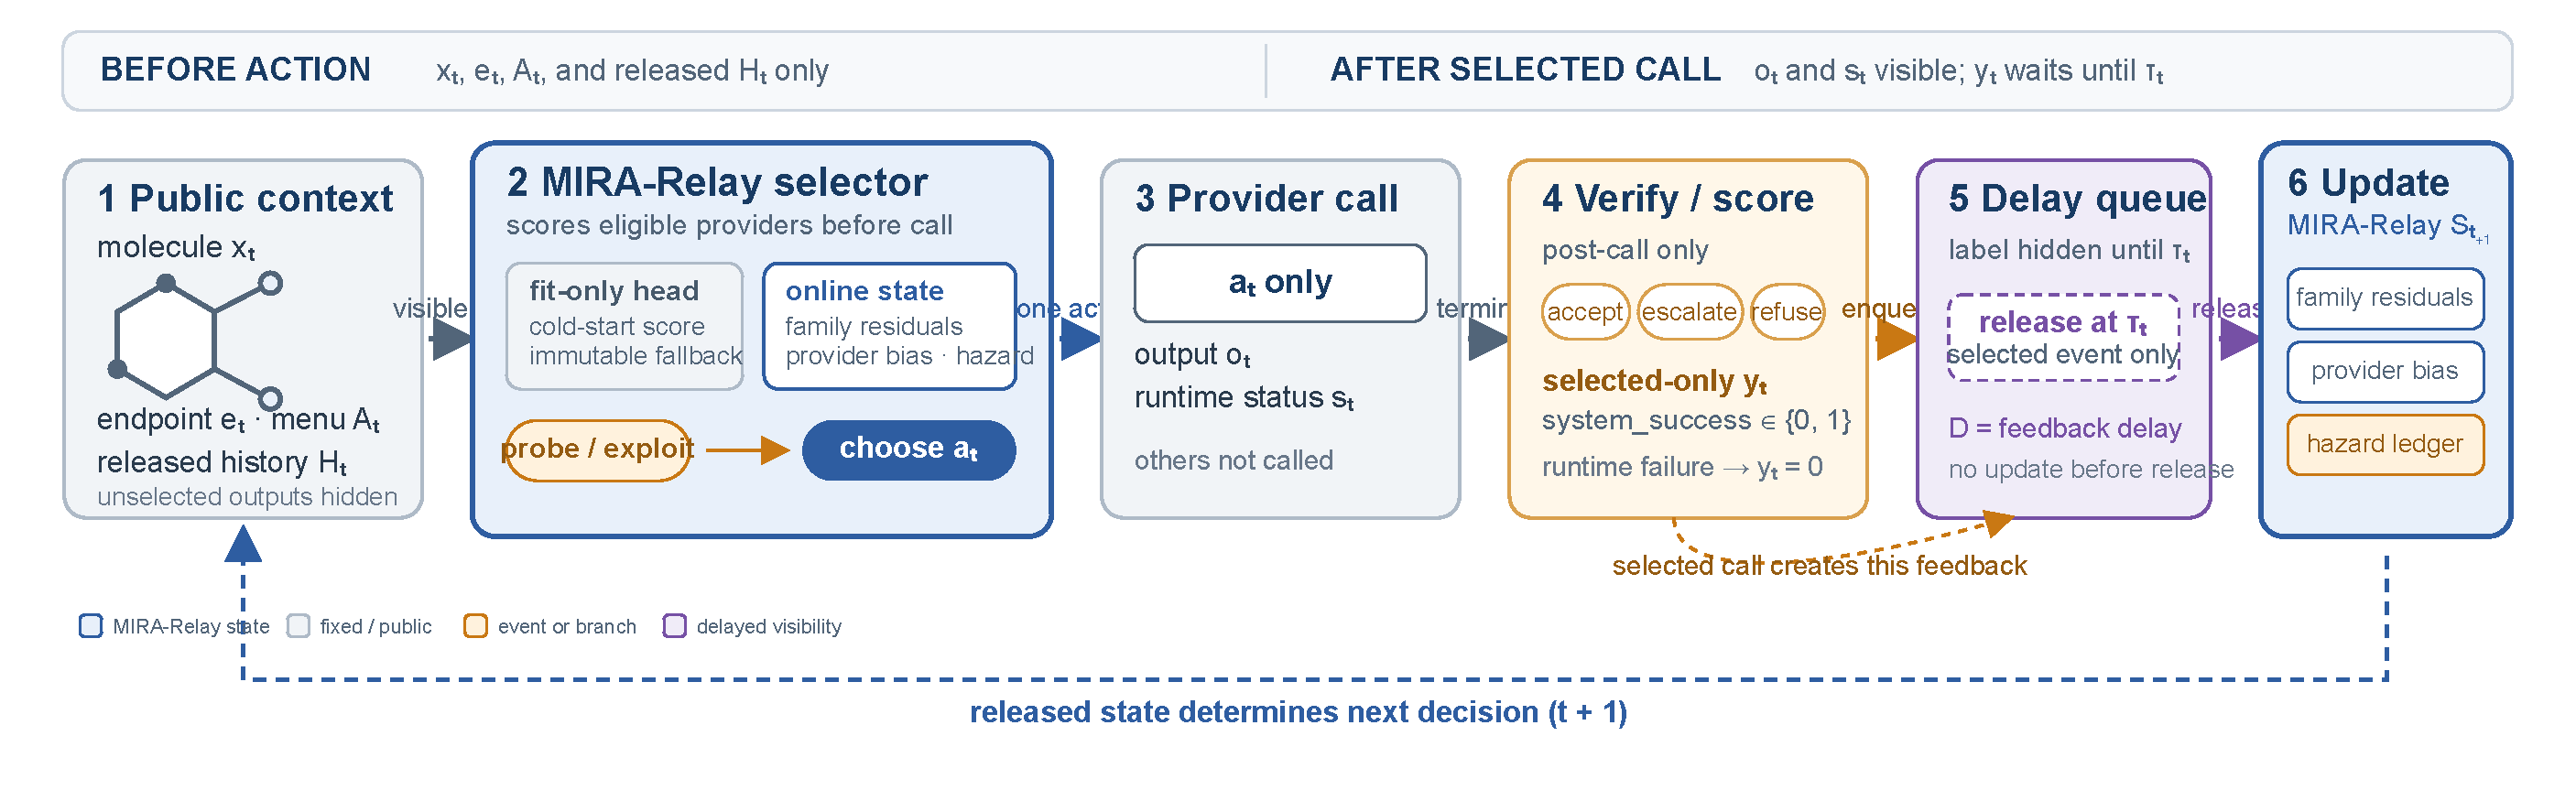
\includegraphics[width=\textwidth]{figures/figure1/v2/figure1_v2.pdf}
  \caption{MIRA-Relay turns tool selection into a delayed event loop. Before action, the selector sees the molecule, endpoint, current provider menu, and released history, then chooses one provider using a fit-only fallback and the online family/provider state. The selected call alone produces a post-call outcome; the label enters a delay queue and updates the state only at its release tick, determining the next choice.}
  \Description{A left-to-right framework with six stages: public molecule and provider-menu context; MIRA-Relay selector with a fit-only direct head, online family residuals and provider bias, and probe/exploit branch; one selected provider call; post-call verifier with accept, escalate, or refuse; a delayed selected-only feedback queue; and a state update containing family residuals, provider bias, and a hazard ledger that feeds the next decision.}
  \label{fig:overview}
\end{figure*}
